% Section 3: Gini Index and Impurity Measures (Slides 19-29)

% Slide 19: How to determine the Best Split?
\begin{frame}{تعیین بهترین تفکیک}{مقایسه شرایط آزمون رقیب}
  \begin{itemize}
    \item \textbf{وضعیت اولیه گره والد:} داده‌های ورودی شامل ۱۰ نمونه با توزیع $C_1: 6$ و $C_2: 4$ است.
    \item کدام ویژگی داده‌ها را به خالص‌ترین زیرمجموعه‌ها تفکیک می‌کند؟
  \end{itemize}
  \vspace{0.15cm}
  \begin{center}
    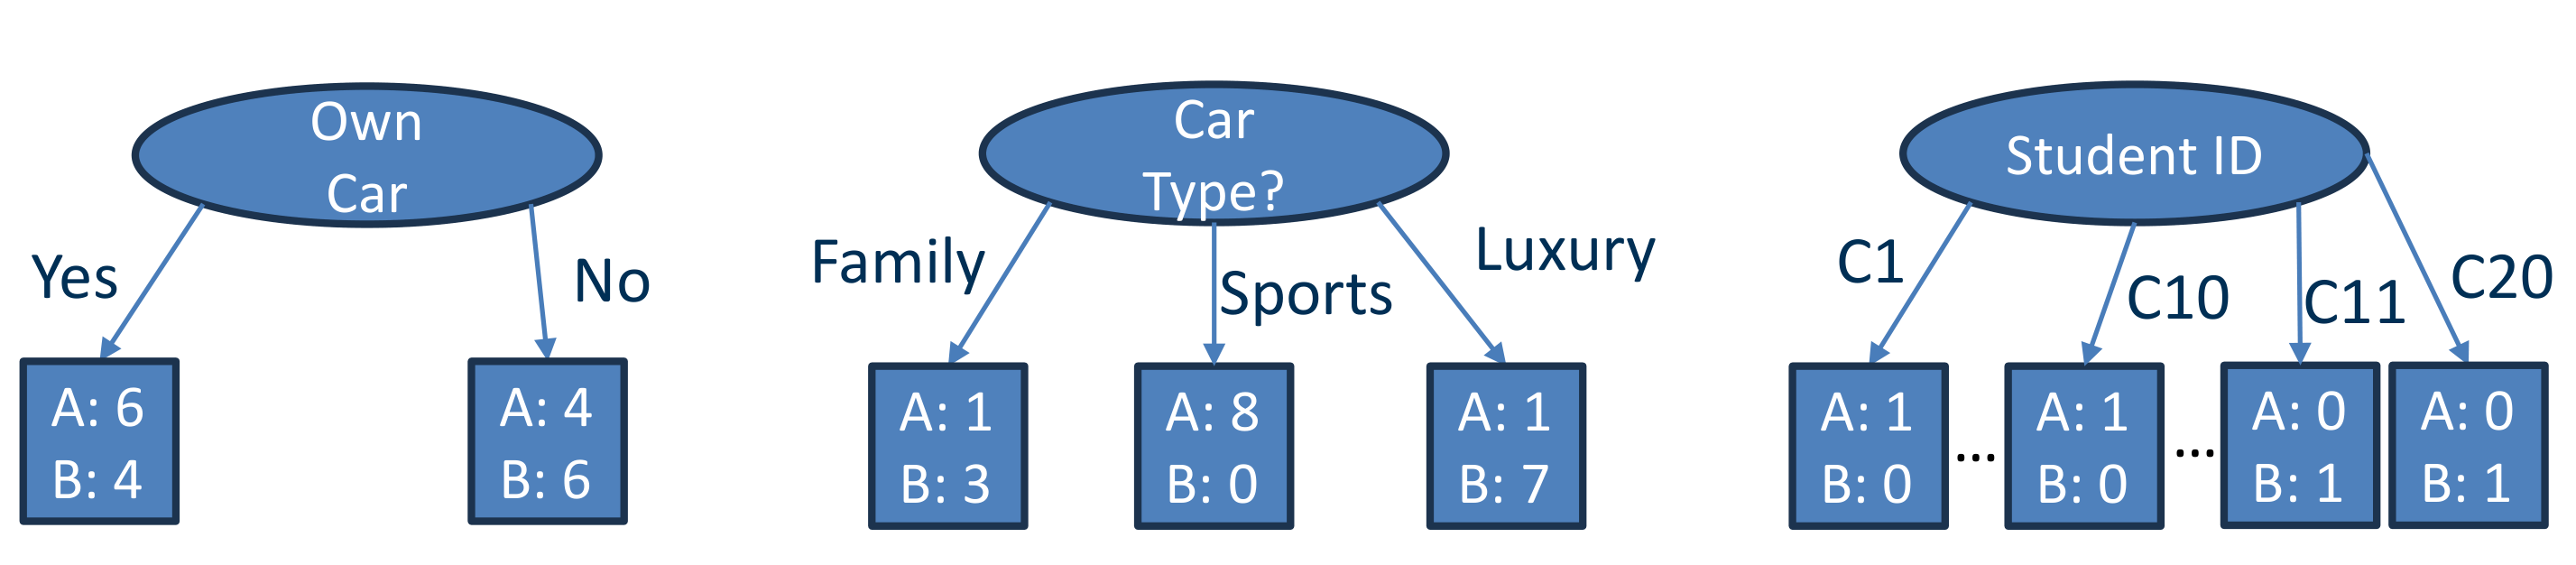
\includegraphics[width=0.96\textwidth,height=4.8cm,keepaspectratio]{images/slide19_split_candidates.png}
  \end{center}
\end{frame}

% Slide 20: Purity and Homogeneity
\begin{frame}{خلوص و همگنی گره‌ها}{مبنای انتخاب شرط تفکیک}
  \begin{itemize}
    \setlength{\itemsep}{7pt}
    \item \textbf{گره‌های همگن (خالص):} گره‌هایی که اکثریت یا تمام نمونه‌های آن‌ها متعلق به یک کلاس واحد هستند.
    \begin{itemize}
      \item در این گره‌ها عدم قطعیت حداقل بوده و خطای طبقه‌بندی بسیار کم یا صفر است.
    \end{itemize}
    \item \textbf{گره‌های ناهمگن (ناخالص):} گره‌هایی با توزیع یکنواخت از کلاس‌های مختلف؛ پیش‌بینی در این گره‌ها بسیار غیرقابل اعتماد است.
    \item \textbf{نیاز به معیار ریاضی:} برای مقایسه دقیق آزمون‌ها به یک معیار کمّی برای اندازه‌گیری \textbf{ناخالصی (\lr{Impurity})} نیاز داریم.
  \end{itemize}
  \vspace{0.15cm}
  \begin{center}
    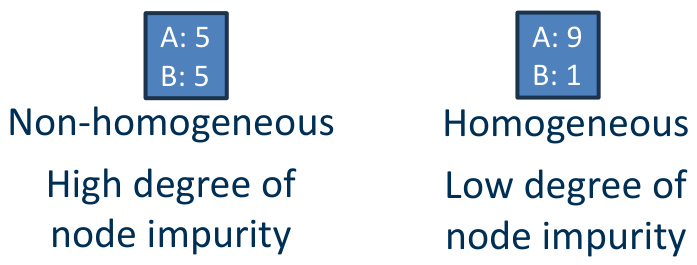
\includegraphics[width=0.75\textwidth,height=2.3cm,keepaspectratio]{images/slide20_node_impurity_clean.png}
  \end{center}
\end{frame}

% Slide 21: Gini Index
\begin{frame}{شاخص جینی}{\lr{Gini Index}}
  \begin{columns}[T]
    \begin{column}{0.66\textwidth}
      \begin{itemize}
        \setlength{\itemsep}{5pt}
        \item \textbf{پیشینه تاریخی:} نام‌گذاری به افتخار \textbf{کورادو جینی (\lr{Corrado Gini}، ۱۸۸۵--۱۹۶۵)}، آماردان برجسته ایتالیایی.
        \item \textbf{کاربرد در اقتصاد:} اندازه‌گیری توزیع ثروت و نابرابری درآمد:
        \begin{itemize}
          \item عدد ۱: یک نفر کل ثروت را دارد (نابرابری مطلق)
          \item عدد ۰: تمام افراد سهم کاملاً برابری دارند (برابری مطلق)
        \end{itemize}
      \end{itemize}
    \end{column}
    \begin{column}{0.30\textwidth}
      \begin{center}
        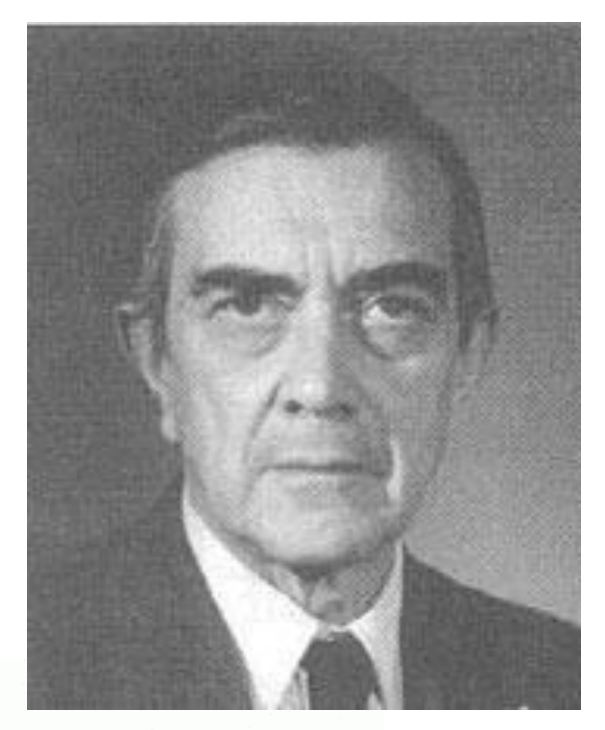
\includegraphics[width=0.85\textwidth,height=2.3cm,keepaspectratio]{images/slide21_gini_portrait.png}\\[0.05cm]
        {\scriptsize\color{subgray}کورادو جینی}
      \end{center}
    \end{column}
  \end{columns}
  \vspace{0.1cm}
  \begin{center}
    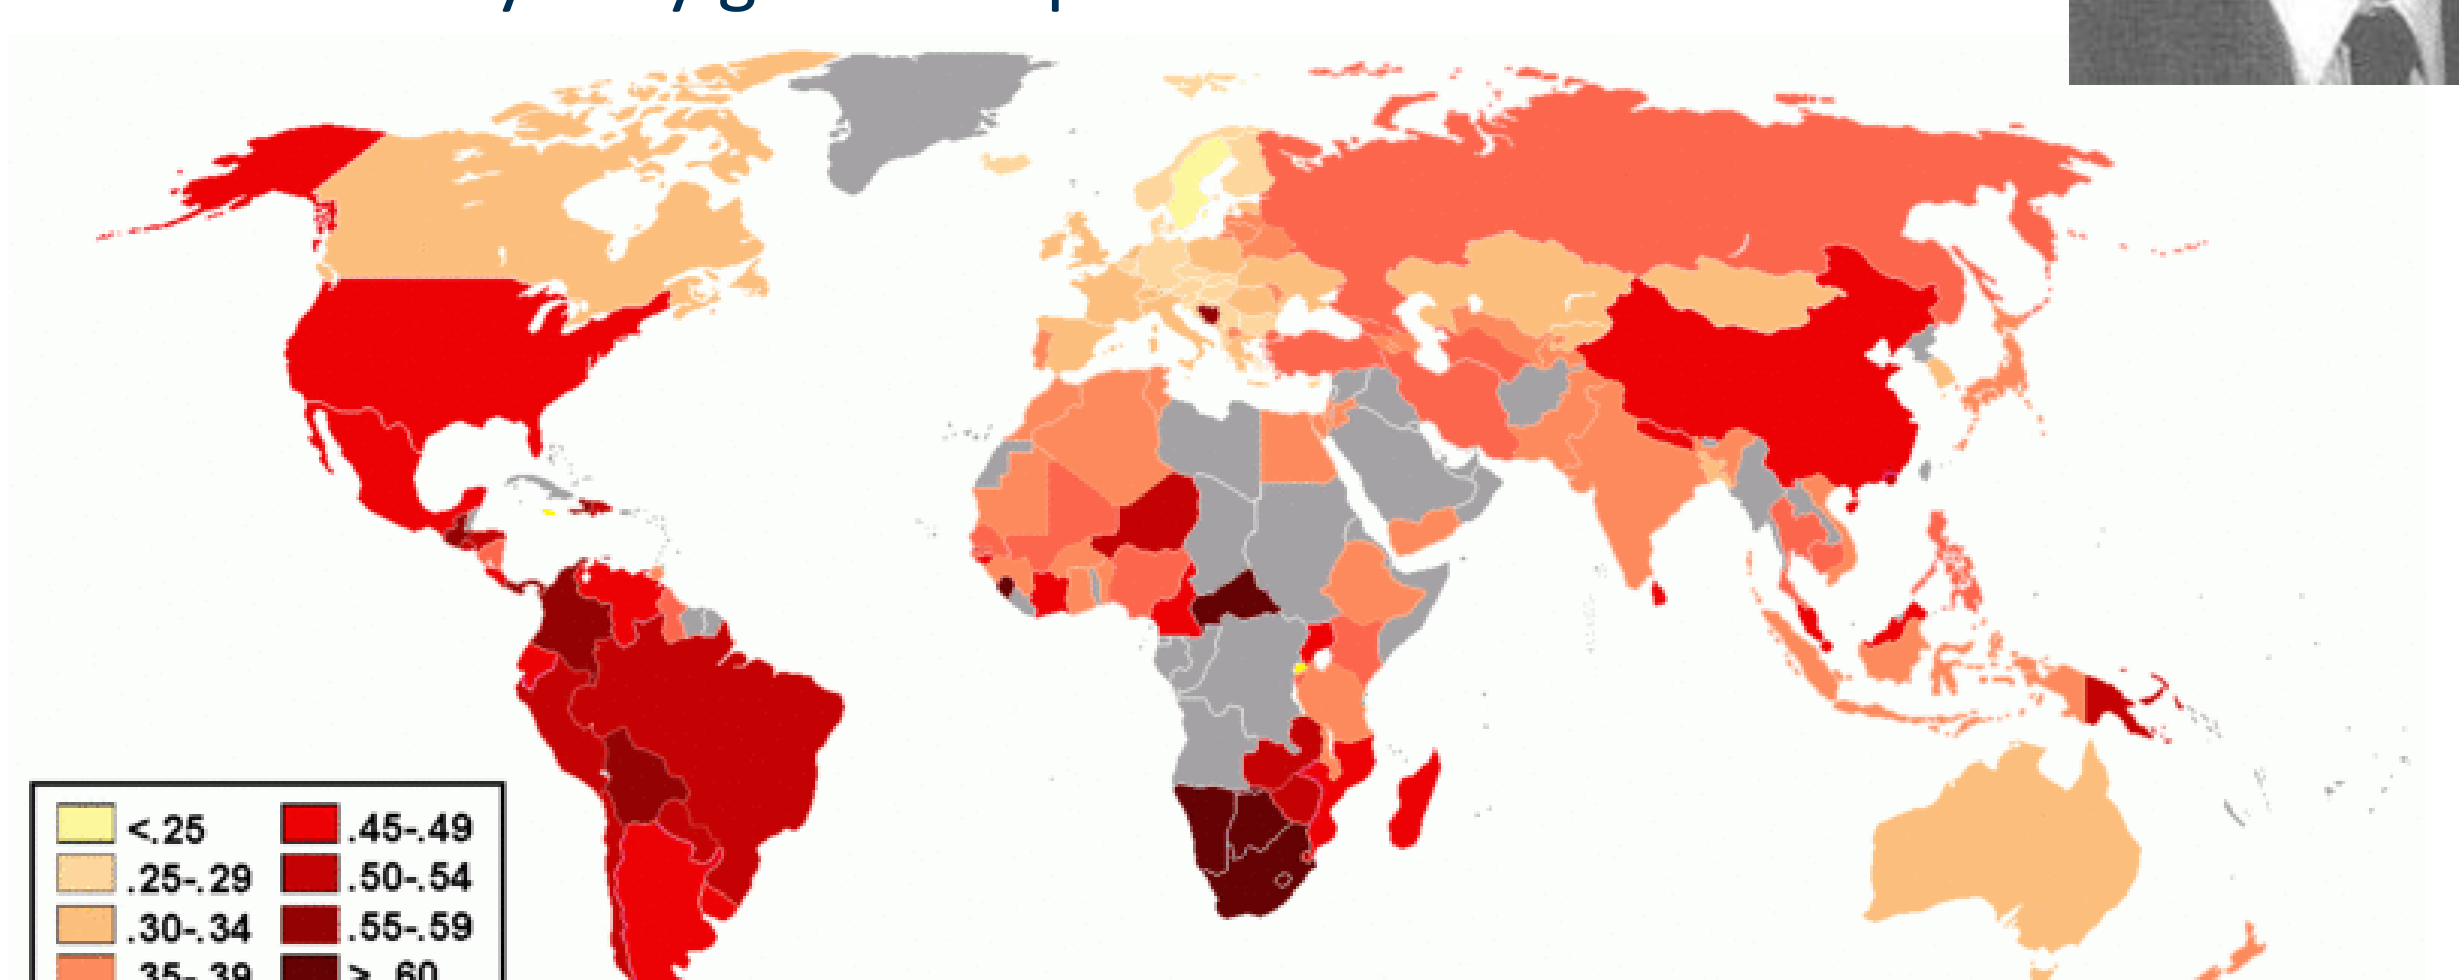
\includegraphics[width=0.92\textwidth,height=2.5cm,keepaspectratio]{images/slide21_gini_world_map.png}
  \end{center}
\end{frame}

% Slide 22: Measure of Impurity: GINI
\begin{frame}{معیار ناخالصی جینی}{\lr{Measure of Impurity: GINI}}
  \begin{itemize}
    \setlength{\itemsep}{4pt}
    \item \textbf{فرمول ریاضی شاخص جینی برای گره مفروض $t$:}
    \[
      \text{GINI}(t) = 1 - \sum_{j} [p(j|t)]^2
    \]
    که در آن $p(j|t)$ نسبت رکوردهای متعلق به کلاس $j$ در گره $t$ است.
    \item \textbf{حداقل ناخالصی ($0.0$):} تمام رکوردها متعلق به یک کلاس هستند (بیشترین اطلاعات).
    \item \textbf{حداکثر ناخالصی ($1 - 1/n_c$):} نمونه‌ها به طور مساوی میان کلاس‌ها تقسیم شده‌اند (کمترین اطلاعات).
  \end{itemize}
  \vspace{0.15cm}
  \begin{center}
    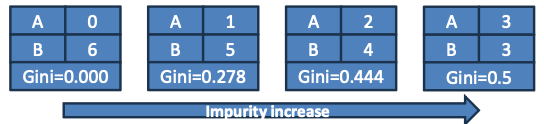
\includegraphics[width=0.88\textwidth,height=2.0cm,keepaspectratio]{images/slide22_gini_impurity_increase_clean.png}
  \end{center}
\end{frame}

% Slide 23: Examples for Computing GINI
\begin{frame}{مثال‌های عددی محاسبه ناخالصی جینی}{\lr{Examples for Computing GINI}}
  \begin{itemize}
    \item محاسبه شاخص جینی برای ۳ گره با درجات خلوص مختلف:
  \end{itemize}
  \vspace{0.1cm}
  \begin{center}
    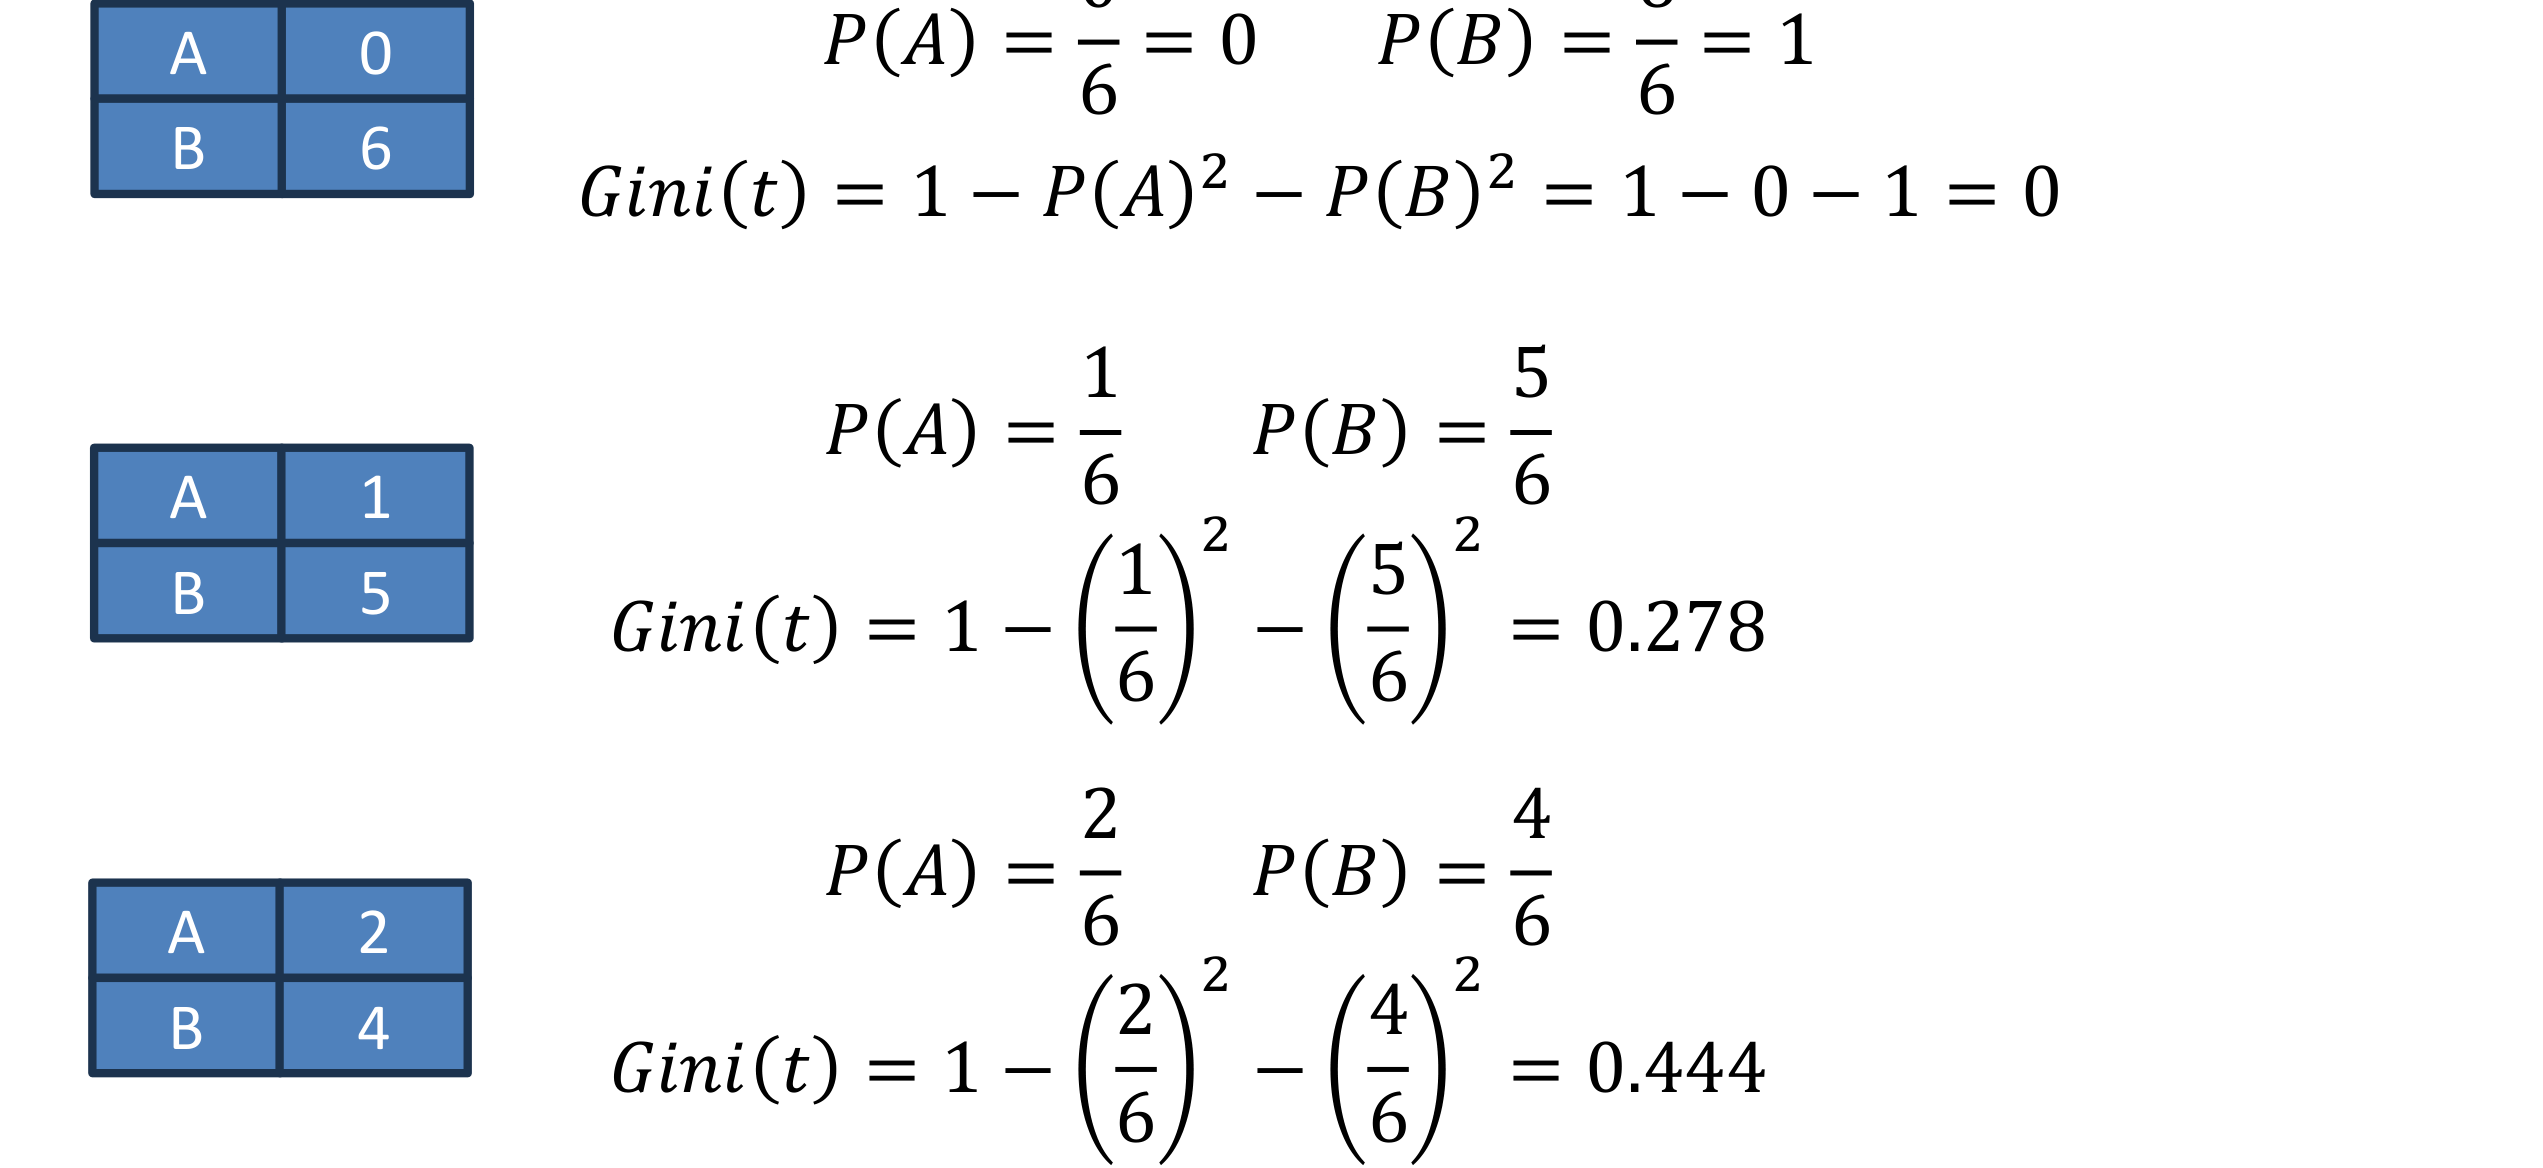
\includegraphics[width=0.92\textwidth,height=4.6cm,keepaspectratio]{images/slide23_gini_clean_examples.png}
  \end{center}
\end{frame}

% Slide 24: Splitting Based on GINI
\begin{frame}{تفکیک بر مبنای شاخص جینی}{\lr{Splitting Based on GINI}}
  \begin{itemize}
    \setlength{\itemsep}{8pt}
    \item هنگامی که گره $p$ به $k$ افراز (گره فرزند) تقسیم می‌شود، کیفیت تفکیک به صورت زیر محاسبه می‌گردد:
  \end{itemize}
  \vspace{0.1cm}
  \begin{center}
    \fcolorbox{mannheimblue}{codebg}{
      \Large $\displaystyle \text{GINI}_{\text{split}} = \sum_{i=1}^{k} \frac{n_i}{n} \text{GINI}(i)$
    }
  \end{center}
  \vspace{0.1cm}
  \begin{itemize}
    \setlength{\itemsep}{5pt}
    \item[] که در آن $n_i$ تعداد رکوردهای گره فرزند $i$ و $n$ تعداد کل رکوردهای گره والد $p$ است.
    \item \textbf{شهود ریاضی:} \lr{(Intuition)} شاخص جینی هر افراز بر اساس اندازه نسبی آن وزن‌دهی می‌شود.
    \item تفکیکی که کمترین مقدار $\text{GINI}_{\text{split}}$ را به همراه داشته باشد، به عنوان تفکیک برنده برگزیده می‌شود.
  \end{itemize}
\end{frame}

% Slide 25: Computing GINI Split
\begin{frame}{محاسبه جینی برای تفکیک دوگانه}{مثال گام‌به‌گام}
  \begin{itemize}
    \item افراز داده‌ها بر اساس ویژگی مالکیت خودرو (\codeinline{Own Car})
  \end{itemize}
  \vspace{0.05cm}
  \begin{center}
    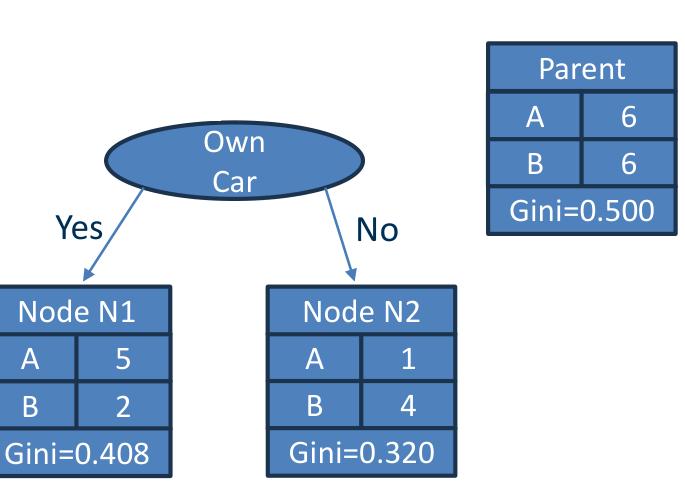
\includegraphics[width=0.68\textwidth,height=2.5cm,keepaspectratio]{images/slide25_gini_car_tree_clean.png}
  \end{center}
  \vspace{-0.1cm}
  \begin{itemize}
    \setlength{\itemsep}{4pt}
    \item \textbf{محاسبه جینی کل تفکیک:}
    \[
      \text{GINI}_{\text{split}} = \frac{7}{12} \times 0.408 + \frac{5}{12} \times 0.320 = \mathbf{0.371}
    \]
    \item \textbf{بهبود خلوص:} \lr{(Purity Gain)}
    \[
      \text{Gain} = \text{GINI}_{\text{parent}} - \text{GINI}_{\text{split}} = 0.500 - 0.371 = \mathbf{0.129}
    \]
    \item در صورت استفاده از آنتروپی، این مقدار \textbf{بهره اطلاعات (\lr{Information Gain})} نامیده می‌شود.
  \end{itemize}
\end{frame}

% Slide 26: Categorical Attributes
\begin{frame}{ویژگی‌های دسته‌ای: محاسبه شاخص جینی}{\lr{Categorical Attributes: Computing Gini}}
  \begin{itemize}
    \item برای هر مقدار مجزا، شمارش کلاس‌ها انجام شده و حالات تفکیک مقایسه می‌شوند:
  \end{itemize}
  \vspace{0.15cm}
  \begin{center}
    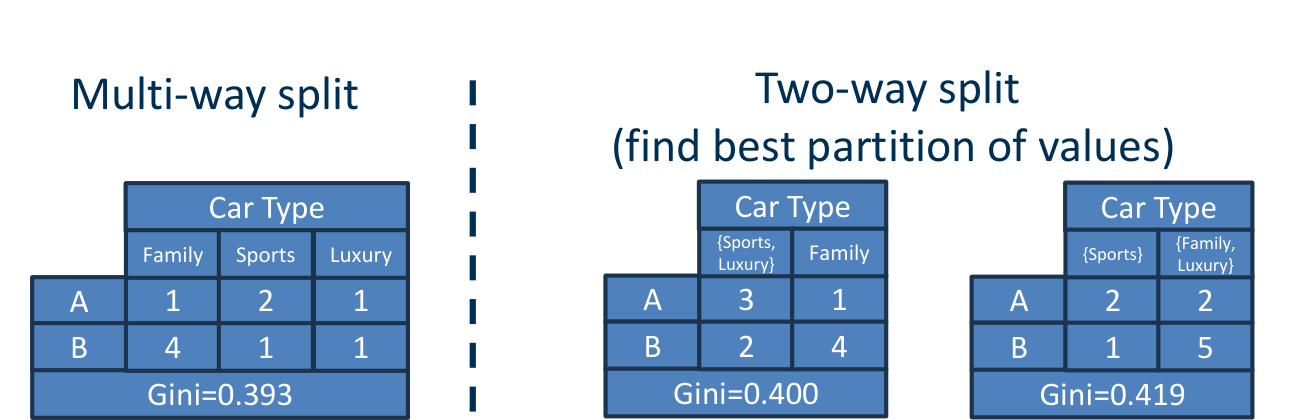
\includegraphics[width=0.92\textwidth,height=4.4cm,keepaspectratio]{images/slide26_categorical_tables_clean.png}
  \end{center}
\end{frame}

% Slide 27: Continuous Attributes
\begin{frame}{ویژگی‌های پیوسته: راهکار ارزیابی}{\lr{Continuous Attributes: Computing Gini}}
  \begin{columns}[T]
    \begin{column}{0.56\textwidth}
      \begin{itemize}
        \setlength{\itemsep}{7pt}
        \item استفاده از تصمیم‌گیری‌های دوگانه بر مبنای یک مقدار آستانه ($A < v$ در برابر $A \ge v$)
        \item \textbf{تعداد گزینه‌های تفکیک:} برابر با تعداد مقادیر مجزای ویژگی در داده‌ها
        \item هر آستانه تفکیک ماتریس شمارش کلاس متناظر با خود را دارد.
        \item \textbf{روش ساده اما ناکارآمد:} پویش کل پایگاه‌داده برای تک‌تک مقادیر و محاسبه مجدد جینی (دارای تکرار زائد و کند).
      \end{itemize}
    \end{column}
    \begin{column}{0.42\textwidth}
      \begin{center}
        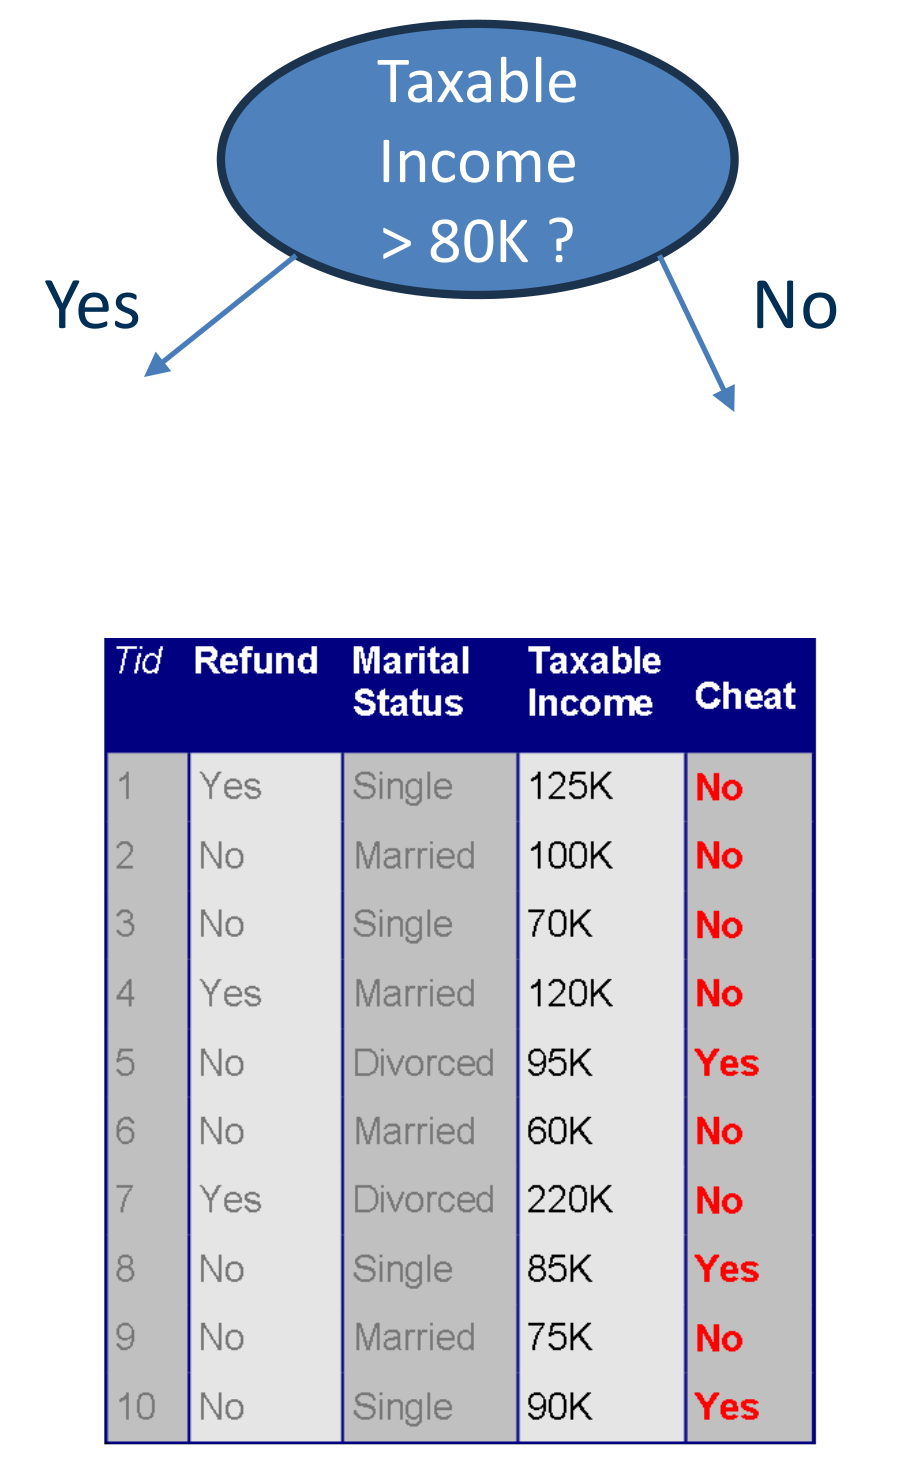
\includegraphics[width=\textwidth,height=5.2cm,keepaspectratio]{images/slide27_continuous_graphic.png}
      \end{center}
    \end{column}
  \end{columns}
\end{frame}

% Slide 28: Continuous Attributes: Efficient Computation
\begin{frame}{ویژگی‌های پیوسته: الگوریتم محاسباتی سریع}{\lr{Continuous Attributes: Efficient Computation}}
  \begin{itemize}
    \setlength{\itemsep}{4pt}
    \item \textbf{رویه کارآمد ۳ مرحله‌ای:}
    \begin{enumerate}
      \setlength{\itemsep}{2pt}
      \item مرتب‌سازی رکوردهای آموزشی بر اساس مقادیر ویژگی ($O(N \log N)$)
      \item پویش خطی مقادیر و به‌روزرسانی تدریجی ماتریس شمارش و جینی در زمان $O(1)$
      \item انتخاب موقعیت تفکیکی که کمترین شاخص جینی را حاصل می‌کند.
    \end{enumerate}
  \end{itemize}
  \vspace{0.1cm}
  \begin{center}
    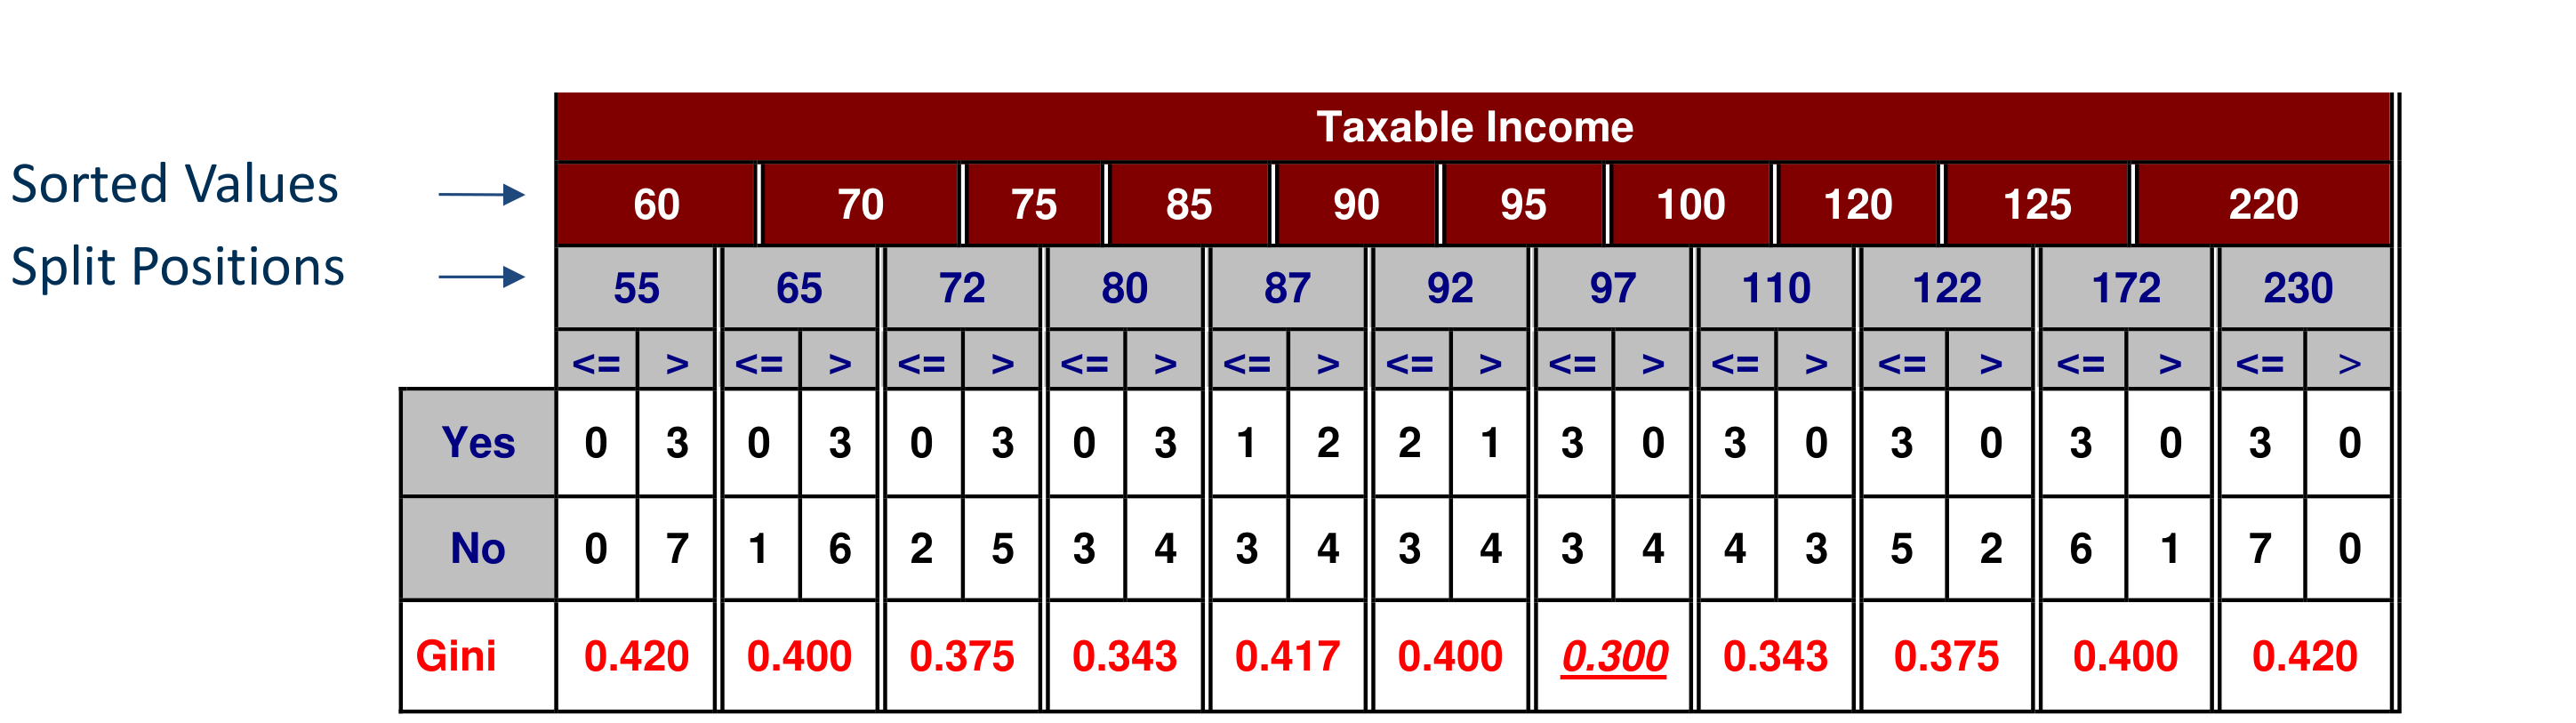
\includegraphics[width=0.96\textwidth,height=3.4cm,keepaspectratio]{images/slide28_continuous_clean_table.png}
  \end{center}
\end{frame}

% Slide 29: Continuous Attributes: Distribution
\begin{frame}{ویژگی‌های پیوسته: محاسبه شاخص جینی}{\lr{Continuous Attributes: Computing Gini Index}}
  \begin{itemize}
    \item \textbf{نکته کلیدی:} محاسبه شاخص جینی تنها برای موقعیت‌هایی که برچسب کلاس تغییر می‌کند، کفایت می‌کند!
  \end{itemize}
  \vspace{0.15cm}
  \begin{center}
    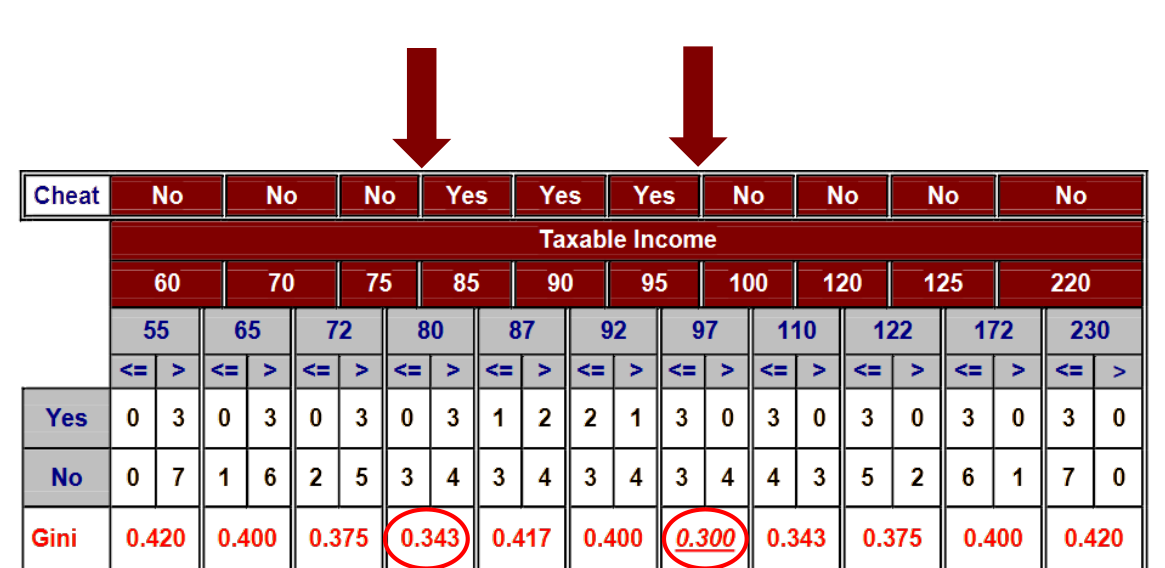
\includegraphics[width=0.95\textwidth,height=4.8cm,keepaspectratio]{images/slide29_continuous_histogram_clean.png}
  \end{center}
\end{frame}
